\documentclass[a0paper,portrait]{baposter}

% Packages

\usepackage[utf8]{inputenc}
\usepackage{url}
\usepackage{booktabs}
\usepackage{amsmath}
\usepackage{amsfonts}
\usepackage{relsize}

\usepackage{enumitem}
\setlist{leftmargin=5mm}

\usepackage{tikz}
\usetikzlibrary{shapes}
\usepgflibrary{fpu}

% Graphics

\graphicspath{{../figures/}}
\definecolor{TUMBlue}{RGB}{0, 94, 184}

% Custom Commands

\newcommand{\aff}{\textsuperscript{$\star$}}
\newcommand{\compresslist}{
\setlength{\itemsep}{1pt}
\setlength{\parskip}{2pt}
\setlength{\parsep}{2pt}
\vspace{-0.75em}
}

% Bibliography

\usepackage[
  backend=biber,
  sorting=nty,
  style=ieee,
  minbibnames=1,
  maxbibnames=1,
  maxcitenames=1,
  mincitenames=1,
  defernumbers=true]{biblatex}
\addbibresource{../lit.bib}

\AtEveryBibitem{%
  \clearfield{url}%
  \clearfield{doi}%
  \clearfield{issn}
  \clearfield{volume}
  \clearfield{number}
  \clearfield{pages}
  \clearfield{isbn}
  \clearfield{eprint}
}

\DefineBibliographyStrings{english}{%
  references = {},
}

\renewcommand\refname{}

% Document

\begin{document}

% Background is white.
% \background

\background{
  \begin{tikzpicture}[remember picture,overlay]%
    \draw (12.75, 7.5) node {\includegraphics[scale=1]{tiled}};
    \draw (12.75, 24) node {\includegraphics[scale=1]{tiled}};

    \draw[white, fill=white, rounded corners=1pt]
         (current page.north west)+(1.5, -0.5)
          rectangle ++(20.5, -3.5);

    \draw[white, fill=white, rounded corners=1pt]
         (current page.north east)+(-3.2, -0.5) rectangle ++(-0.3, -3.2);

  \end{tikzpicture}
}


\begin{poster}{
  grid=false,
  eyecatcher=true,
  borderColor=white,
  headerColorOne=TUMBlue,
  headerColorTwo=TUMBlue,
  headerFontColor=white,
  boxColorOne=white,
  headershape=smallrounded,
  background=user,
  headerborder=none,
  textborder=none,
  boxshade=plain,
  headerheight=100pt
}
{
  % Eye Catcher
}
{
  {\bf CytoGAN: Generative Modeling of Cell Images}
  \vspace{3mm}
}
%%% Authors %%%%%%%%%%%%%%%%%%%%%%%%%%%%%%%%%%%%%%%%%%%%%%%%%%%%%%%%%%%%%%%%%%%
{
  \smaller[0.5]
  \hspace{-3mm}Peter Goldsborough\textsuperscript{$\star$\,\textdagger}, Nick Pawlowski\textsuperscript{$\ddagger$}, Juan C. Caicedo\aff, Shantanu Singh\aff, Anne E. Carpenter\aff

  \vspace{2mm}
  {
    \smaller[1]
    \textsuperscript{$\star$} Broad Institute of MIT and Harvard \hspace{3mm}%
    \textdagger\hspace{2pt} Technical University Munich \hspace{3mm}%
    $\ddagger$ Imperial College London
  }
}
% Logos
{
  \begin{tabular}{l}
    \includegraphics[width=0.1\textwidth]{broad-logo}\\
    \vspace{-2mm}\\
    \includegraphics[width=0.1\textwidth]{imperial-logo}
    \vspace{-2mm}\\
    \includegraphics[width=0.1\textwidth]{tum-logo}\\
  \end{tabular}
}

\headerbox{Introduction}{name=intro, column=0, row=0}{

\emph{Morphological profiling} aims to map microscopy images of perturbed cells to salient vector representations that divide the morphological space into clusters of cells with similar properties or function.

\vspace{2mm}

Current approaches are divided between a) classical image processing, requiring manual fine-tuning and expert knowledge b) transfer learning with deep CNNs trained on miscellaneous objects, allowing no domain-specific adaptation.

\vspace{2mm}

Instead, we model cells with \emph{Generative Adversarial Networks} (GANs) for both representation learning and cell synthesis. Advantages of our approach are:
\vspace{2mm}
\begin{itemize}
\compresslist
\item \textbf{Unsupervised} representation learning, which can readily incorporate new data;
\item \textbf{Specialization} to training data, allowing identification of the semantic relations between biologically meaningful channels;
\item \textbf{Interpretability} of learned representations and useful visualization that help translate data variations into meaningful biological phenotypes.
\end{itemize}
}

\headerbox{Exploring Biological Phenotypes Using Cell Synthesis}{name=synth, span=2, column=1, row=0}{

Besides learning salient representations of microscopy cell images, GANs allow us to synthesize cell images and explore variations in the noise and learned latent spaces. This allows biologically meaningful experiments and improves interpretability of our method.

\vspace{-1mm}
\begin{center}
  \begin{tikzpicture}
      \foreach \i/\kind in {0/began, 1/bigan, 2/lsgan, 3/real, 4/wgan} {
        \foreach \j in {0} {
          \draw ({\i * 3}, {\j * 1.5})
          node {\includegraphics[width=2cm, height=2cm]{generated/\kind/\j}};
        }
      }
  \end{tikzpicture}
\end{center}
\vspace{-2mm}

Shown above are cells synthesized with LSGAN, WGAN, BEGAN and BiGAN
architectures alongside a real cell. The synthesized images are not only highly
detailed and realistic, but also consistent with their biological nature. For
example, it is characteristic that $\beta$-Tubulin (green channel) forms a
circular halo cradling the nucleus. This property is maintained clearly in all
generated images. }

\headerbox{Interpolating Cell Images in Noise and Latent Space}{name=interpol, span=2, column=1, row=1, below=synth}{

GANs are known to learn low manifolds of their input priors, such that
interpolation between two points $\mathbf{z}_1, \mathbf{z}_2$ drawn from the noise space $P_{\text{noise}}$ results in visually smooth
transitions in generated images. We confirm that this property holds for
microscopy cell images.

\vspace{-1mm}
\begin{center}
\begin{tikzpicture}
  \foreach \i in {0, 1} {
    \foreach \j in {0, ..., 9} {
      \draw ({\j * 1.5}, {\i * -1.5}) node
      {\includegraphics[width=1.5cm, height=1.5cm]{noise-interpolation/\i/\j}};
    }

  }
\end{tikzpicture}
\end{center}
\vspace{-2mm}

Bidirectional GANs (BiGAN\cite{}) extend the vanilla DCGAN architecture with an
explicit encoder network that enables both synthesis of images from noise
\emph{and} inference of latent representations, in such a way that the noise and
latent space are fused. This means we can encode real cell images, perturb,
transform or, in this case, interpolate between them, and re-synthesize the
resulting vectors.

\vspace{-2mm}
\begin{center}
\begin{tikzpicture}
    \foreach \i in {0, ..., 9} {
      \draw ({\i * 1.5}, 0) node
      {\includegraphics[width=1.5cm, height=1.5cm]{latent-interpolation/\i}};
    }

    \fill[black] (0.25, -0.75) rectangle ++(12, 2mm);
\end{tikzpicture}
\end{center}
}

\headerbox{Vector Algebra for Biological Interpretability}{name=algebra, span=2, column=1, row=1, below=interpol}{

We find that GANs partition the noise space into regions capturing different semantic properties of cells, allowing biologically meaningful algebra on noise vectors.

\vspace{-3mm}
\begin{center}
\begin{tikzpicture}
    \draw (0, 0) node {\includegraphics[scale=0.4]{algebra/figure-chan}};
    \draw (-3.7, -1.2) node {\footnotesize Much $\beta$-Tubulin}
        ++(2.5, 0) node {\footnotesize Little $\beta$-Tubulin}
        ++(2.5, 0) node {\footnotesize Any Cell}
        ++(2.5, 0) node {\footnotesize More $\beta$-Tubulin}
        ;

    % \draw (0, -2.5) node {\includegraphics[scale=0.4]{algebra/figure-nucl}};
    % \draw (-3.7, -3.7) node {\footnotesize Large Nucleus}
    %     ++(2.5, 0) node {\footnotesize Small Nucleus}
    %     ++(2.5, 0) node {\footnotesize Any Cell}
    %     ++(2.5, 0) node {\footnotesize Larger Nucleus}
        ;
\end{tikzpicture}
\end{center}
\vspace{-3mm}

When the noise and learned latent space are fused (BiGAN), algebra on real cell images becomes possible. This open the door to discovery of a whole new class of highly interpretable and biologically valuable relationships, such as:

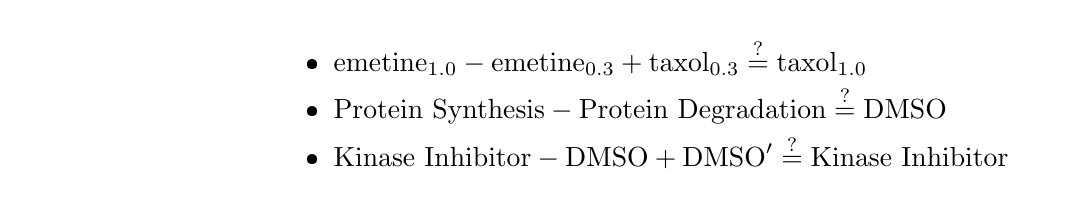
\begin{tikzpicture}
  \draw (-8, 0);
  \draw (0, 0) node [text width=10cm] {
  \begin{itemize}
    \compresslist
    \item $\text{emetine}_{1.0} - \text{emetine}_{0.3} + \text{taxol}_{0.3} \stackrel{?}{=} \text{taxol}_{1.0}$
    \item $\text{Protein Synthesis} - \text{Protein Degradation} \stackrel{?}{=} \text{DMSO}$
    \item $\text{Kinase Inhibitor} - \text{DMSO} + \text{DMSO}' \stackrel{?}{=} \text{Kinase Inhibitor}$
  \end{itemize}
  };
\end{tikzpicture}
\vspace{2.5pt}
}

\headerbox{Representation Learning for Morphological Profiling}{name=rep, span=2, column=1, row=1, below=algebra}{

We investigate the ability of GANs to learn vector representations of cell
images and evaluate their quality quantitatively at the task of
mechanism-of-action (MOA) prediction. We train a variety of GAN models on 1.3
million microscopy images of cells perturbed with particular drug compounds,
average signatures across treatments and predict the MOA via nearest-neighbor
classification.

\vspace{2mm}
\begin{tikzpicture}
  \draw (-2, 0);
  \draw (0, 0.3) node {\includegraphics[scale=0.2, trim={4cm 3.5cm 8cm 3cm}, clip]{latent-space}};
  \draw (7.75, 1.2) node [text width=11cm, align=justify] {
  For WGAN and LSGAN we interpret the activations of the penultimate dense
  layer as a source of representations. BEGAN an BiGAN architectures already have explicit inference modules. We find that while GANs
  are superior to autoencoders, they are not yet competitive with existing
  classical or deep transfer-learning techniques.
  };

  \draw (8, -1) node [text width=10.5cm] {
    \begin{tabular}{ccccc}
      \toprule
      LSGAN & BiGAN & VAE \cite{pawlowski2016msc} & CP \cite{Singh2014} & Transfer Learning \cite{ando2017improving} \\
      \midrule
      68\% & 70\%& 49\% & 90\% & 96\% \\
      \bottomrule \\
    \end{tabular}
  };
\end{tikzpicture}
\vspace{-6mm}
}

\headerbox{Code \& Data}{name=code, column=0, row=1, below=intro}{Code and experiments are available at \url{github.com/goldsborough/cytogan}. Our data is the BBBC021 dataset from the Broad BioImage Benchmark Collection (\url{data.broadinstitute.org/bbbc/BBBC021/}).}

\headerbox{Acknowledgements}{name=ack, column=0, row=2, below=code}{
We thank Mike Ando and Google, Inc. for providing computational resources to accelerate our research. We also thank all members of the Broad Imaging Platform for fruitful discussion and their continuous guidance and support.
}
\headerbox{References}{name=ref, column=0, row=3, below=ack}{
\printbibliography
}

\end{poster}
\end{document}
